\documentclass{article}

\usepackage[letterpaper, portrait, margin=1.5in]{geometry}

\usepackage{fancyhdr}
\usepackage{ragged2e}
\usepackage{graphicx}
\usepackage{caption}
\usepackage{amsmath}
\usepackage{rotating}

\usepackage{listings}
\usepackage{color}

\definecolor{dkgreen}{rgb}{0,0.6,0}
\definecolor{gray}{rgb}{0.5,0.5,0.5}
\definecolor{mauve}{rgb}{0.58,0,0.82}

\lstset{frame=tb,
  language=Java,
  aboveskip=3mm,
  belowskip=3mm,
  showstringspaces=false,
  columns=flexible,
  basicstyle={\small\ttfamily},
  numbers=none,
  numberstyle=\tiny\color{gray},
  keywordstyle=\color{blue},
  commentstyle=\color{dkgreen},
  stringstyle=\color{mauve},
  breaklines=true,
  breakatwhitespace=true,
  tabsize=4
}

\setcounter{secnumdepth}{1}

\usepackage{chngcntr}
\counterwithin{figure}{section}

\renewcommand*{\thepage}{C\arabic{page}}

\pagestyle{fancy}
\lhead{ACME Robotics}
\chead{\#8367}
\rhead{\ifcontents Contents \else Week \thesection \fi}

\newif\ifcontents
\contentstrue

\makeatletter
\renewcommand{\@seccntformat}[1]{}
\makeatother
\begin{document}

\subsection{Changing the Intake Arm Length and Whip Stiffness}
The team had planned on increasing the intake arm length for a while because of the idea that it could allow for longer arms and a farther reach. The reason it wasn't done yet was because there was trouble with finding the right length belts for the changed length. Fortunately Kelly found the right belts and ordered them. Meanwhile Ashlin manufactured the new arms, that were one inch longer, to work with the belts when they arrived. Once the belts arrived, Aidan and Ashlin got to work putting them on and testing. They found that they had to change the angle of the arms in order for the whips not to hit the ground. With the desired changes in place they tested the setup. Aidan also found that if they changed all the chips on the third roller to the thicker whip material intaking in auto would also become easier. You can see the cut out intake arms in Figure \ref{fig:intakearms} and the final whips and arms can be seen in Figure \ref{fig:arms}. The result was the intake was able to grab minerals a lot faster and whip them up with a greater velocity.

\begin{figure}
    \centering
    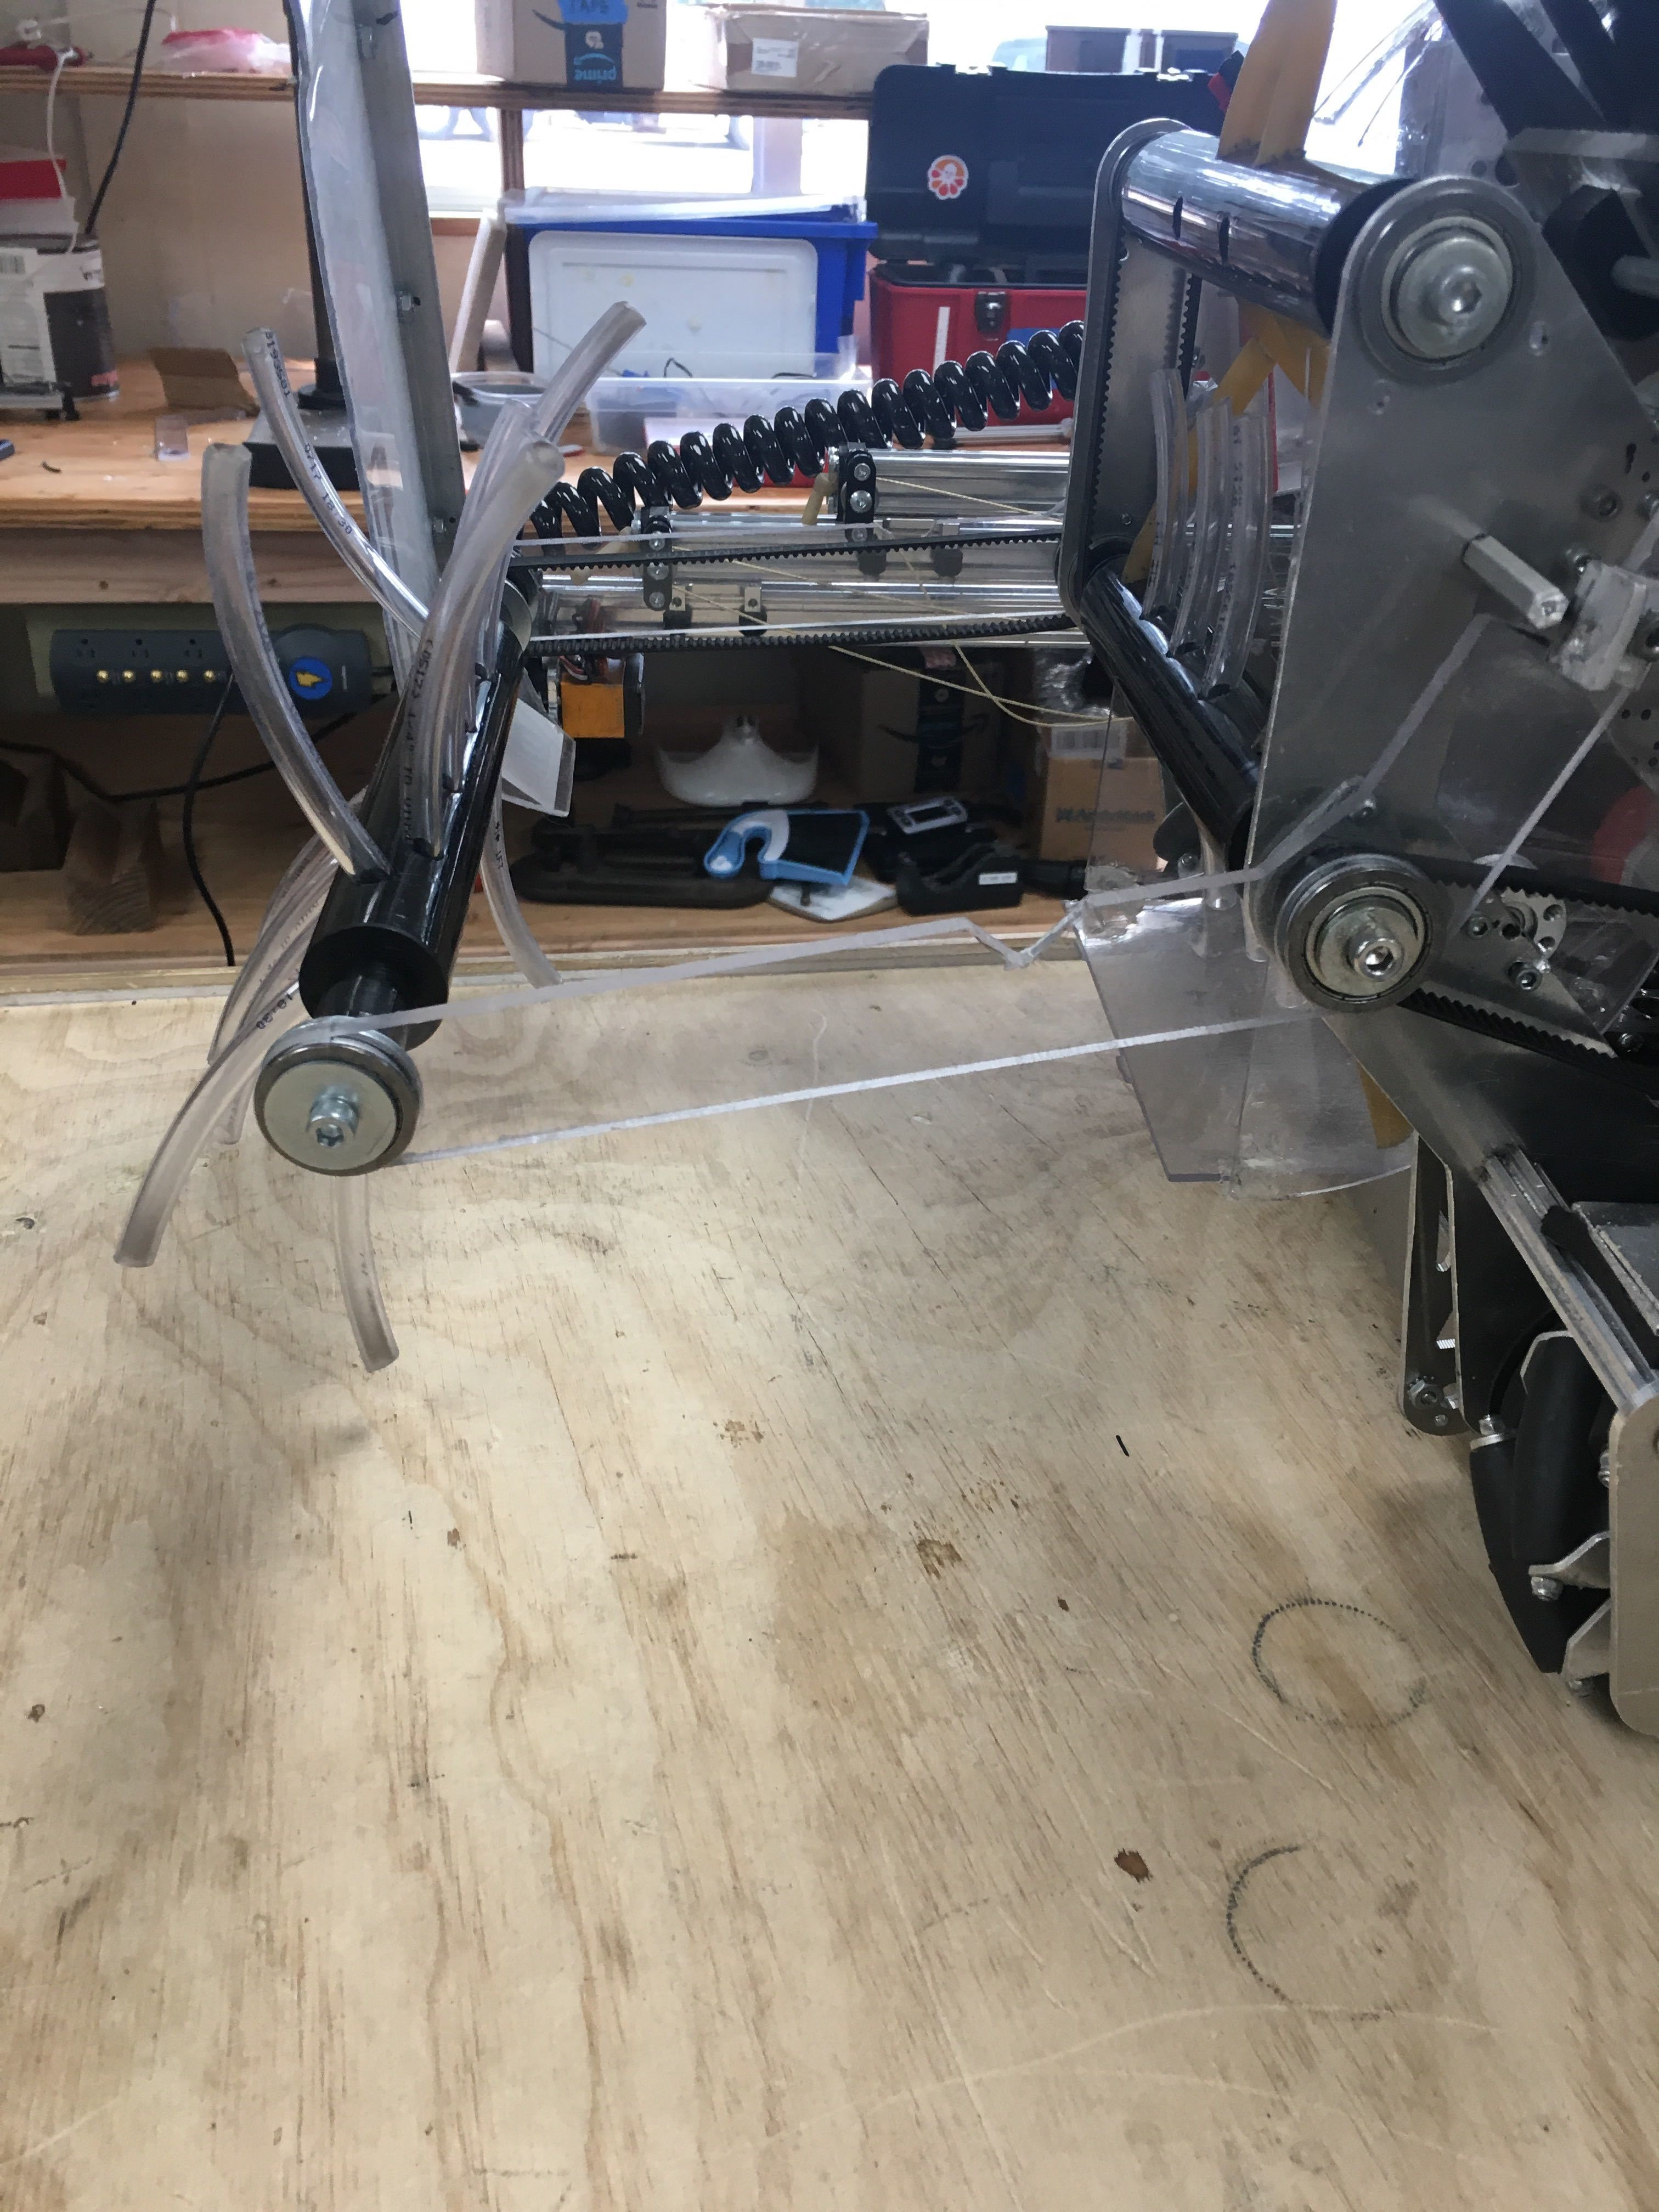
\includegraphics[width= 0.5 \textwidth]{31_04-01/images/IMG_1934.JPG}
    \caption{New Intake Arms and Whips}
    \label{fig:arms}
\end{figure}

\begin{figure}
    \centering
    \includegraphics[width= 0.5 \textwidth]{31_04-01/images/intakearms.jpg}
    \caption{New Intake Arms}
    \label{fig:intakearms}
\end{figure}

\end{document}